% SBrT Model adapted for the group project
\documentclass[english,hidelinks]{sbrt}
\usepackage[english]{babel}
\usepackage[utf8]{inputenc}
\usepackage{graphicx}
\usepackage{subfigure}
\usepackage{amsmath}
\usepackage{url}
\usepackage{cite}
\usepackage{float}
\usepackage{hyperref}
\usepackage{caption}
\captionsetup{
  font=footnotesize,
  labelsep=period,
  format=plain,
  justification=raggedright,
  singlelinecheck=false
}

\begin{document}
\title{Paper Level Monitoring System in Dispensers Using Ultrasonic Sensor and MQTT Protocol}
\author{Arthur Peixoto Schiller, Franc Wang, and Juliana de Oliveira\\IBMEC - Embedded Systems and IoT}
\maketitle

\markboth{XLIII BRAZILIAN SYMPOSIUM ON TELECOMMUNICATIONS AND SIGNAL PROCESSING - SBrT 2025, SEPTEMBER 29TH TO OCTOBER 2ND, NATAL, RN}{}

\begin{abstract}
This work presents the development of a prototype system for real-time monitoring of paper level in dispensers, using an ultrasonic sensor and MQTT protocol communication. The main goal is to reduce user dissatisfaction caused by lack of paper replacement, especially in high-traffic locations. The sensor detects the paper level and automatically sends alerts to the maintenance staff whenever critical values are reached. The proposed system is low-cost, easy to replicate, and highly scalable. Information is visualized through a mobile app developed with React Native.
\end{abstract}
\begin{keywords}
Monitoring, Dispenser, Ultrasonic Sensor, MQTT, IoT.
\end{keywords}

\section{Introduction}
We currently live in the \textbf{Experience Era}, where companies must offer unique experiences to customers, going beyond simply delivering products or services. Factors such as cleanliness, organization, and the availability of essential items directly influence the perception of quality and comfort, impacting customer retention and willingness to return. User experience has become a fundamental pillar for business success. In this context, we propose a system to monitor the paper level in dispensers using an ultrasonic sensor and MQTT communication. When the paper is running low, the system issues an alert, allowing for timely replacement before the paper runs out.

\section{System Description}
The system consists of:
\begin{itemize}
    \item HC-SR04 ultrasonic sensor (up to 4 meters range);
    \item ESP32 CP2103 microcontroller;
    \item Communication via MQTT protocol using Mosquitto broker;
    \item Mobile app developed in React Native with Expo and JavaScript;
    \item Paho-MQTT library for MQTT integration;
    \item Battery-powered (under testing);
    \item Sending frequency: 200 ms.
\end{itemize}
The distance sensor is positioned at the top of the dispenser, measuring the distance to the top of the paper stack. When the dispenser is full, this distance is minimal; as paper is removed, the distance increases. When 70\% of the total height is reached, the system interprets this as a critical limit and issues a replacement alert. Communication is performed via MQTT, segmented into three topics: current paper percentage, descriptive status ("full", "needs refill" or "empty"), and the distance value in centimeters. Notifications are sent only under critical conditions, optimizing data traffic.

\begin{figure}[H]
  \centering
  \fbox{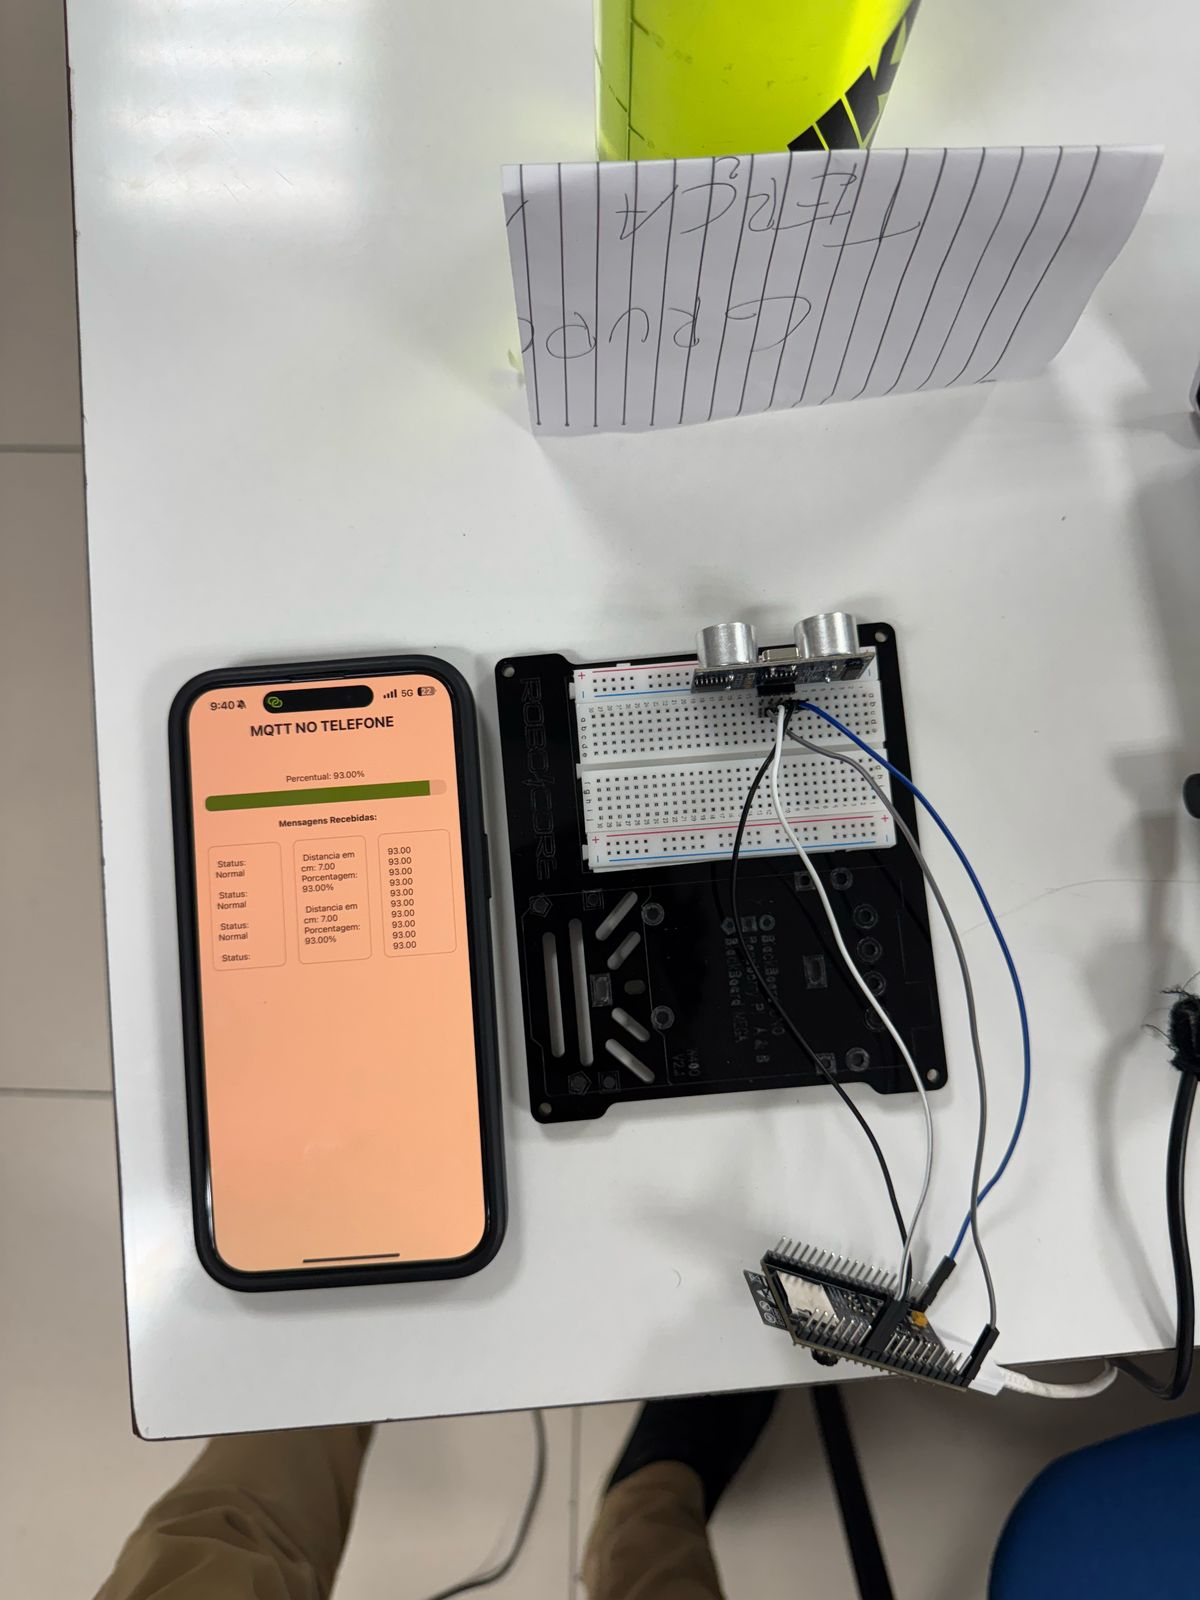
\includegraphics[width=0.4\textwidth]{montagemSistema.jpg}}
  \caption{Prototype of the system installed with ultrasonic sensor and ESP on a test bench.}
  \label{fig:sistema}
\end{figure}

\section{Testing and Validation}
Three bench tests were conducted in a laboratory environment. The results indicated moderate accuracy in the measurements, sufficient to validate the functional feasibility of the system. As part of the remote monitoring architecture, a mobile app was developed with React Native, communicating with the embedded system via MQTT, allowing real-time visualization of dispenser status. The web interface simplifies monitoring and decision-making.

Future technical directions:
\begin{itemize}
    \item Improvements to the web interface layout, focusing on responsiveness;
    \item Administrative dashboard for multiple devices;
    \item Implementation of visual and sound alerts for critical events.
\end{itemize}

\begin{figure}[H]
  \centering
  \fbox{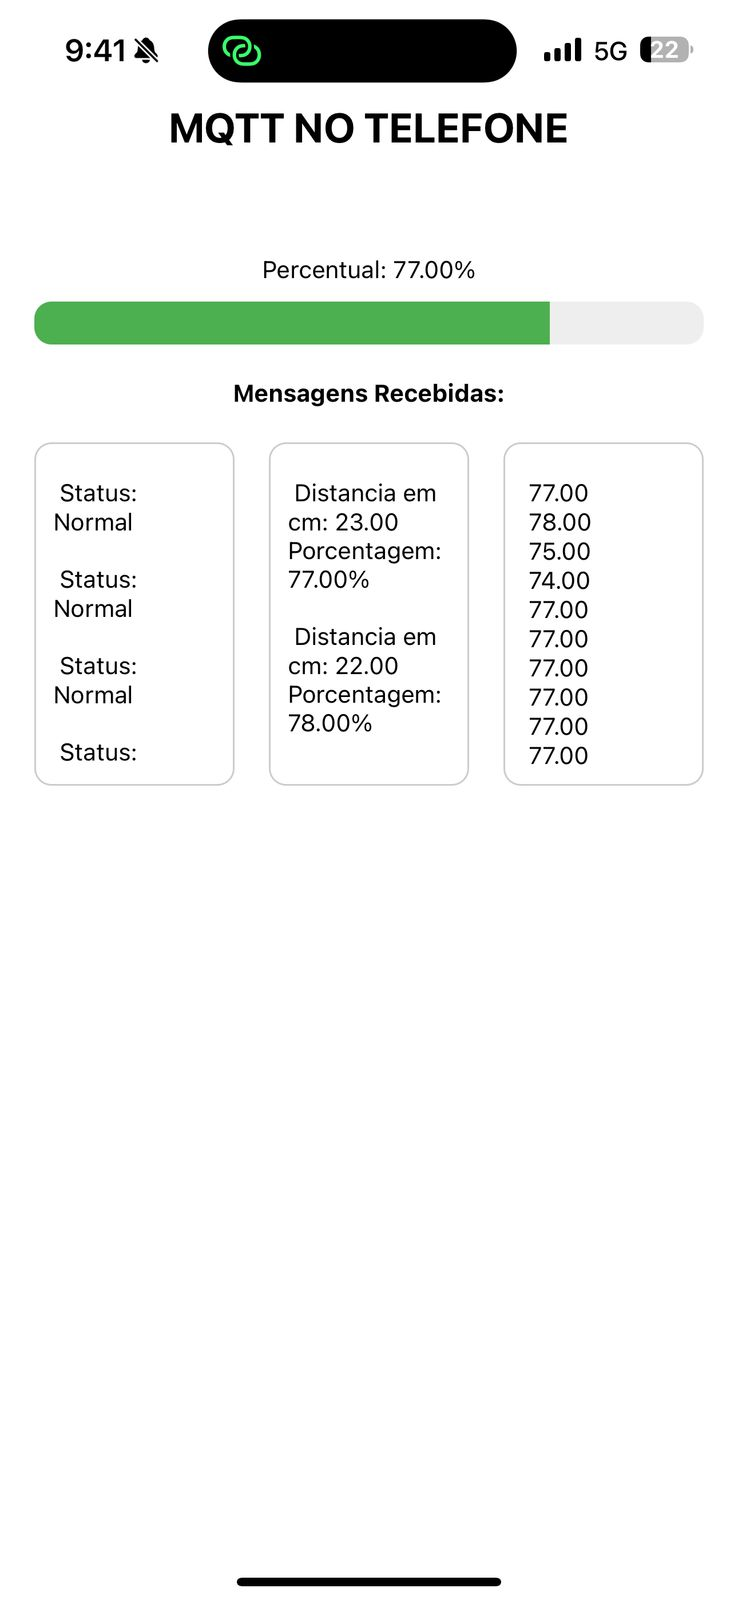
\includegraphics[width=0.3\textwidth]{printApp.jpg}}
  \caption{Main screen of the app developed for monitoring data via MQTT.}
  \label{fig:app}
\end{figure}

\section{Experimental Results and Quantitative Performance}
To assess the system's accuracy and repeatability, five experiments were conducted with the ultrasonic sensor, varying the distance from the paper to the sensor (2, 7, 12, 17, and 22 cm). Each test generated a set of 500 samples, analyzed quantitatively as described below.

\textbf{Note:} The ultrasonic sensor used has low accuracy for distances less than 2 cm. Therefore, in the experiments, the 20 cm dispenser was tested with the paper positioned at least 2 cm from the sensor, avoiding the low-performance range and ensuring greater reliability in the measurements.

% Smaller graphics for up to 3 pages

% Boxplot of Distances
\begin{figure}[H]
    \centering
    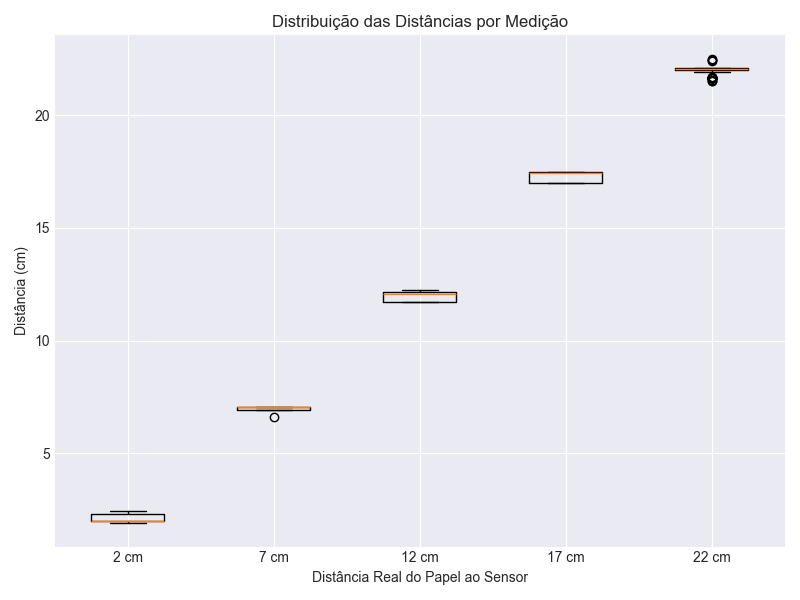
\includegraphics[width=0.28\textwidth]{graficos/boxplot_distancias.png}
    \caption{Boxplot of sensor readings for different paper-to-sensor distances.}
    \label{fig:boxplot_distancias}
\end{figure}

% Standard Deviation of Measurements
\begin{figure}[H]
    \centering
    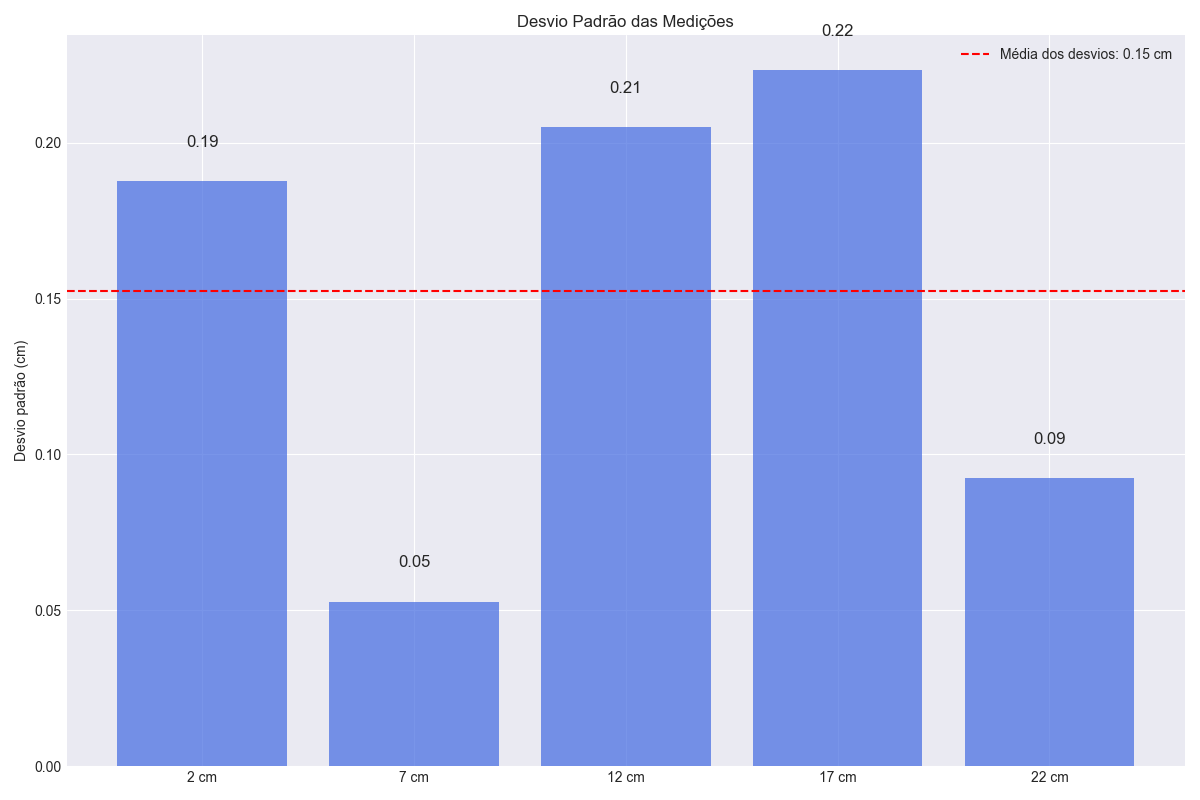
\includegraphics[width=0.28\textwidth]{graficos/desvios_padrao.png}
    \caption{Standard deviation of sensor readings for each paper position.}
    \label{fig:desvios_padrao}
\end{figure}

% Temporal Evolution of Readings
\begin{figure}[H]
    \centering
    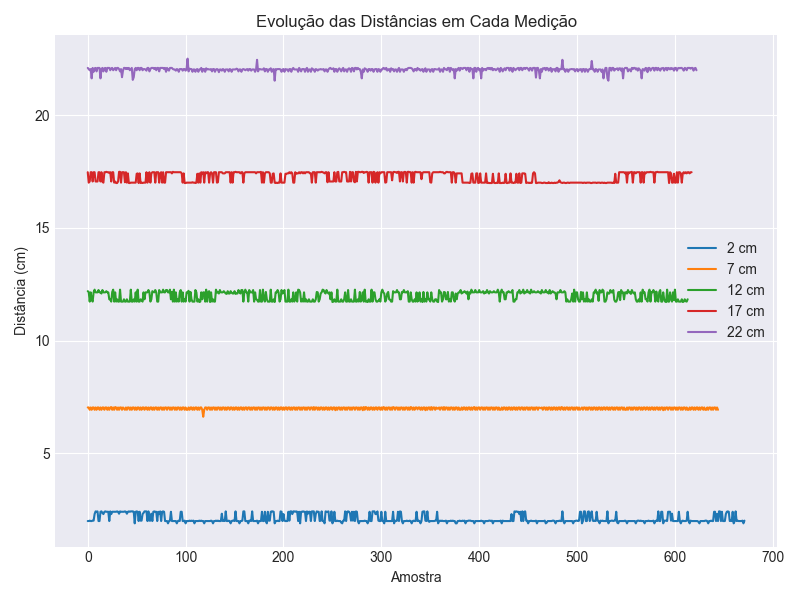
\includegraphics[width=0.28\textwidth]{graficos/series_temporais.png}
    \caption{Temporal evolution of sensor readings for different distances.}
    \label{fig:series_temporais}
\end{figure}

% Amplitude of Measurements
\begin{figure}[H]
    \centering
    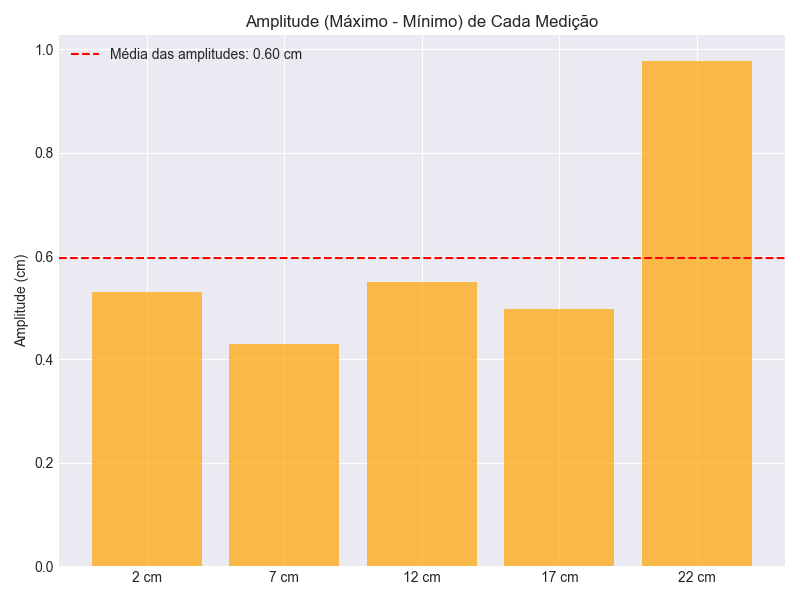
\includegraphics[width=0.28\textwidth]{graficos/amplitudes.png}
    \caption{Amplitude of sensor readings for each paper position.}
    \label{fig:amplitudes}
\end{figure}

\subsection{Percent Error Rate}
The overall system accuracy was evaluated by the mean absolute percentage error (MAPE), comparing the mean readings with the actual distance. Figure~\ref{fig:erro_percentual} shows the percent error for each test and the global MAPE (red line), which remained low in all conditions, indicating excellent performance for stock monitoring applications.

\begin{figure}[H]
    \centering
    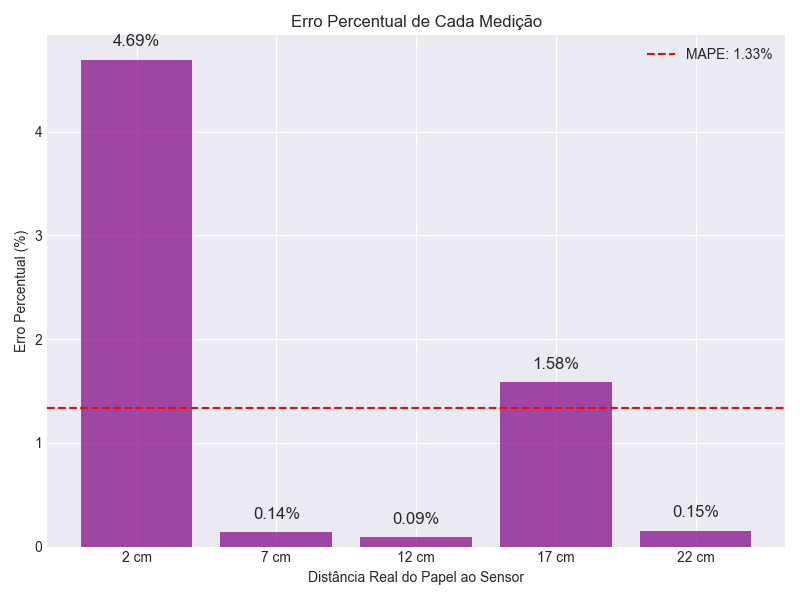
\includegraphics[width=0.45\textwidth]{graficos/erro_percentual.png}
    \caption{Mean percent error of system measurements compared to actual distances.}
    \label{fig:erro_percentual}
\end{figure}

These results demonstrate that the system offers high accuracy, low variability, and excellent reliability for monitoring paper level in dispensers, making it suitable for real IoT and stock control applications.

\section{Conclusion}
The experimental results showed that the developed system provides high accuracy and reliability for monitoring paper level in dispensers. The mean absolute percentage error (MAPE) obtained in the tests was low, and the mean absolute error was around a few millimeters to 1 cm, even across different sensor operating ranges. Considering that stock control of paper does not require millimeter precision, this error is absolutely negligible for the proposed application. In practice, small variations do not impact efficient paper replacement, ensuring that alerts are issued reliably and without false alarms. Therefore, the system fully meets the requirements for automated monitoring, being robust, low-cost, and easily replicable for real environments. The use of ultrasonic sensors, combined with quantitative data analysis, proved to be an effective solution for IoT applications focused on real-time supply control.

\textbf{Note:} The ultrasonic sensor used has low accuracy for distances less than 2 cm. Therefore, in the experiments, the 20 cm dispenser was tested with the paper positioned at least 2 cm from the sensor, avoiding the low-performance range and ensuring greater reliability in the measurements.

\bibliographystyle{IEEEtran}
% \bibliography{refs} % Uncomment and adjust if references are available

\end{document}
